%% Week 48 -- the last week.  Monday lecture, 2 x 45 min, in two parts.
%% Lecture 1: summary of decision trees and ensemble methods (weeks 46-47,
%% Chapter 7): one tree, bagging, random forests, AdaBoost, gradient boosting,
%% XGBoost -- the whole ladder applied to two real data sets, the Wisconsin
%% breast-cancer data (classification) and the California housing data
%% (regression).  Lecture 2: summary of the semester, weeks 34-47, built on
%% the 2025 summary lecture (doc/src/week48/week48.do.txt): what we covered,
%% the threads that connect the methods, practical advice, perspectives.
%% No Tuesday session this week; lab only Wednesday November 25, 12:15-16:00,
%% dedicated to Project 3 (deadline Monday December 14).
%% Figures: week48_*.pdf from make_week48_figures.py; exam1.jpeg and
%% Nebbdyr2.png from doc/src/week48/figures.  Companion notebook: week48.ipynb.
%% Book references (book.aux 2026-10-25): Chapter 7 -- Eqs 7.1 (tree), 7.7
%% (Gini), 7.8 (entropy), 7.9 (CART cost), 7.12 (node MSE), 7.16 (variance of
%% an average), 7.17 (out-of-bag), 7.18 (m ~ sqrt p), 7.19-7.20 (additive
%% model, stagewise), 7.26-7.29 (AdaBoost), 7.30 (functional gradient), 7.33-7.37
%% (XGBoost); Eq. 2.52 (bias-variance); Chapter 18 = concluding remarks.
%% Build:  pdflatex week48slides.tex  (twice)
\documentclass[10pt,aspectratio=169]{beamer}
\usetheme{red_plain}
\usepackage[T1]{fontenc}
\usepackage[utf8]{inputenc}
\usepackage{amsmath,amssymb,bm}
\usepackage{graphicx}
\usepackage{listings}
\usepackage{xcolor}
\usepackage{booktabs}
\usepackage{array}
\newcolumntype{L}[1]{>{\raggedright\arraybackslash}p{#1}}
\usepackage{tikz}
\usetikzlibrary{positioning,arrows.meta}
\graphicspath{{./}{../../src/week48/figures/}}

%% ---- code listings
\definecolor{codebg}{rgb}{0.97,0.97,0.97}
\lstset{language=Python,basicstyle=\ttfamily\scriptsize,backgroundcolor=\color{codebg},
  keywordstyle=\color{blue!70!black}\bfseries,commentstyle=\color{green!45!black},
  stringstyle=\color{red!60!black},showstringspaces=false,frame=single,
  framerule=0pt,xleftmargin=4pt,xrightmargin=4pt,breaklines=true,columns=fullflexible}

%% ---- the "pause and think" question frames
\newcounter{insight}
\newenvironment{insight}[1][]{%
  \stepcounter{insight}%
  \begin{frame}{Pause and think \arabic{insight}: #1}%
  \setbeamercolor{block title}{bg=structure.fg,fg=white}%
  \setbeamercolor{block body}{bg=structure.fg!8}%
  \small
}{\end{frame}}
\newcommand{\question}[1]{\begin{block}{Question}#1\end{block}}
\newcommand{\answer}[1]{\pause\begin{block}{Answer}#1\end{block}}

\setbeamertemplate{footline}[frame number]
\setbeamerfont{block title}{size=\small}
\setbeamertemplate{blocks}[rounded][shadow=false]
\setbeamercovered{invisible}

\newcommand{\var}{\mathrm{var}}
\newcommand{\err}{\overline{\mathrm{err}}}
\newcommand{\sgn}{\mathrm{sign}}

\title{Week 48: Trees and Ensembles in One Lecture, and the Semester in Another}
\subtitle{First lecture: one tree, many trees in parallel, many trees in
  sequence -- on two real data sets.\\ Second lecture: what we have done from
  week 34 to week 47, and what connects it}
\author{Morten Hjorth-Jensen}
\institute{Department of Physics and Center for Computing in Science Education,\\
  University of Oslo, Norway}
\date{}

\begin{document}

\begin{frame}
\titlepage
\end{frame}

\begin{frame}{Plan for week 48 -- the last week}
\footnotesize
\begin{columns}[T]
\begin{column}{0.56\textwidth}
\textbf{Monday November 23, first lecture: decision trees and ensemble
methods, weeks 46 and 47 in one go.}
\begin{enumerate}
  \item The ladder from a single tree to XGBoost, and what each step
    repairs.
  \item \textbf{Classification}: the whole ladder on the Wisconsin
    breast-cancer data.
  \item \textbf{Regression}: the same on the California housing data,
    with the bias and the variance of every step measured.
  \item What to tune, and when to use what.
\end{enumerate}
\textbf{Second lecture: summary of the course, weeks 34--47.}
\begin{enumerate}\setcounter{enumi}{4}
  \item What we have covered, week by week.
  \item Four threads that run through all of it.
  \item One function and one data set, all the methods.
  \item \textbf{The insights we want you to have.}
  \item Practical advice for a machine-learning project.
  \item What we left out; from our methods to reinforcement learning and
    language models; other courses.
\end{enumerate}
\end{column}
\begin{column}{0.42\textwidth}
\begin{block}{This week}
\begin{itemize}
  \item \textbf{No Tuesday session.}
  \item \textbf{Lab only on Wednesday November 25, 12:15--16:00}, dedicated
    to work on \textbf{Project 3}.
  \item Project 3: deadline \textbf{Monday December 14} at midnight.  The
    updated rules for the use of LLMs are at the beginning of the project
    text.
  \item No weekly exercises: the Project-3 proposal of week 47 was the last
    one.
\end{itemize}
\end{block}
\textbf{Reading}: Chapter 7 (all of it) for the first lecture; Chapter 18,
\emph{Concluding remarks and perspectives}, for the second.

\textbf{Code}: \texttt{week48.ipynb} and \texttt{make\_week48\_figures.py}
contain everything behind the figures and numbers of today.
\end{column}
\end{columns}
\end{frame}

%% =====================================================================
\section{Lecture 1: trees and ensembles}
%% =====================================================================

\begin{frame}{}
\centering
{\Large\textbf{First lecture}}\\[6pt]
{\large Decision trees and ensemble methods:\\ from a single tree via
bagging and random forests to boosting}\\[14pt]
\small Chapter 7 -- the material of weeks 46 and 47 -- applied to one data
set for classification and one for regression
\end{frame}

\begin{frame}{The ladder in one picture}
\centering
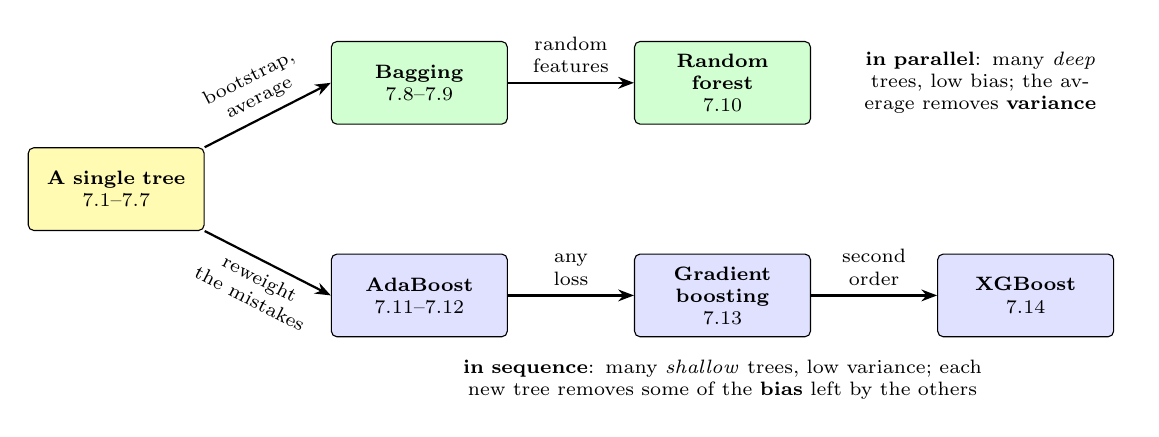
\begin{tikzpicture}[>={Stealth[length=2mm]},
  box/.style={draw,rounded corners=2pt,align=center,minimum height=1.05cm,text width=2.0cm,font=\scriptsize},
  lab/.style={font=\scriptsize,align=center}]
\node[box,fill=yellow!30] (tree) at (0,0) {\textbf{A single tree}\\ 7.1--7.7};
\node[box,fill=green!18] (bag) at (3.85,1.35) {\textbf{Bagging}\\ 7.8--7.9};
\node[box,fill=green!18] (rf) at (7.7,1.35) {\textbf{Random forest}\\ 7.10};
\node[box,fill=blue!12] (ada) at (3.85,-1.35) {\textbf{AdaBoost}\\ 7.11--7.12};
\node[box,fill=blue!12] (gb) at (7.7,-1.35) {\textbf{Gradient boosting}\\ 7.13};
\node[box,fill=blue!12] (xgb) at (11.55,-1.35) {\textbf{XGBoost}\\ 7.14};
\draw[->,thick] (tree.north east) -- (bag.west) node[midway,above,sloped,lab] {bootstrap,\\ average};
\draw[->,thick] (bag) -- (rf) node[midway,above,lab] {random\\ features};
\draw[->,thick] (tree.south east) -- (ada.west) node[midway,below,sloped,lab] {reweight\\ the mistakes};
\draw[->,thick] (ada) -- (gb) node[midway,above,lab] {any\\ loss};
\draw[->,thick] (gb) -- (xgb) node[midway,above,lab] {second\\ order};
\node[lab,anchor=west,text width=3.6cm] at (9.05,1.35) {\textbf{in parallel}: many \emph{deep}
  trees, low bias; the average removes \textbf{variance}};
\node[lab,anchor=north,text width=9cm] at (7.7,-2.05) {\textbf{in sequence}: many \emph{shallow} trees,
  low variance; each new tree removes some of the \textbf{bias} left by the others};
\end{tikzpicture}

\medskip
\small
\begin{columns}[T]
\begin{column}{0.48\textwidth}
\textbf{One tree}: boxes in feature space, a constant in each box.  Readable,
fast, no scaling needed -- and unstable: a deep tree follows the noise, a
shallow one is too coarse.
\end{column}
\begin{column}{0.48\textwidth}
\textbf{Every ensemble} is the same object,
$f(\bm{x})=\sum_{m}\beta_m T_m(\bm{x})$.  The whole difference is how the
trees $T_m$ and the weights $\beta_m$ are chosen.
\end{column}
\end{columns}
\end{frame}

\begin{frame}{Step 0: a single tree (Sections 7.1--7.7)}
\begin{columns}[T]
\begin{column}{0.53\textwidth}
\footnotesize
\begin{block}{The model: $J$ boxes $R_j$, one constant per box, Eq.\ (7.1)}
\[
f(\bm{x})=\sum_{j=1}^{J}c_j\,I(\bm{x}\in R_j),
\]
with $c_j$ the mean $\overline{y}_{R_j}$ (regression) or the majority class
(classification) of the training points in $R_j$.
\end{block}
\begin{block}{The algorithm: CART, greedy recursive binary splitting}
At a node with $m$ points try every feature $k$ and threshold $t$; keep the
pair that minimises the size-weighted impurity of the two children,
\[
C(k,t)=\frac{m_{\mathrm{left}}}{m}\,Q_{\mathrm{left}}
      +\frac{m_{\mathrm{right}}}{m}\,Q_{\mathrm{right}},\tag{7.9}
\]
with $Q$ the Gini index $\sum_kp_k(1-p_k)$, Eq.\ (7.7), the entropy
$-\sum_kp_k\log_2p_k$, Eq.\ (7.8), or for regression the node MSE
$\frac1m\sum_i(y_i-\overline{y})^2$, Eq.\ (7.12).  Then recurse.
\end{block}
\end{column}
\begin{column}{0.45\textwidth}
\footnotesize
\begin{block}{What a tree gives}
\begin{itemize}
  \item a model one can read;
  \item no scaling: invariant to monotone transformations of a feature;
  \item interactions for free -- a split inside a split.
\end{itemize}
\end{block}
\begin{block}{What it costs}
\begin{itemize}
  \item piecewise constant, axis-aligned, no extrapolation;
  \item \textbf{high variance}: $\sigma^2/n_m$ in a leaf with $n_m$ points,
    and the partition itself changes with the data;
  \item the depth is a bias--variance knob with a poor optimum (Runge
    function: best tree $0.0181$, polynomial $0.0133$, noise $0.0100$).
\end{itemize}
\end{block}
\end{column}
\end{columns}
\end{frame}

\begin{frame}{Steps 1 and 2: average many deep trees (Sections 7.8--7.10)}
\begin{columns}[T]
\begin{column}{0.5\textwidth}
\footnotesize
\begin{block}{Why averaging helps: Eq.\ (7.16)}
$B$ predictors, each with variance $\sigma^2$, pairwise correlation $\rho$:
\[
\var\Big(\frac1B\sum_{b=1}^Bf_b\Big)=\rho\,\sigma^2+\frac{1-\rho}{B}\,\sigma^2 .
\]
The second term dies with $B$; the floor $\rho\sigma^2$ does not.  The
expectation -- and therefore the bias -- is that of a single member.
\end{block}
\begin{block}{Bagging (7.9)}
Draw $B$ bootstrap samples, grow one \emph{deep} tree on each, average
(regression) or vote (classification).  Each tree leaves out a fraction
$(1-1/n)^n\approx e^{-1}=0.37$ of the data, Eq.\ (7.17): the
\textbf{out-of-bag} points are a free test set.
\end{block}
\end{column}
\begin{column}{0.48\textwidth}
\footnotesize
\begin{block}{Random forests (7.10)}
Bagged trees all split on the same strong features first and are
correlated.  At every split, let only $m$ randomly chosen features compete:
$m\approx\sqrt{p}$ for classification, Eq.\ (7.18), and $m\approx p/3$ for
regression.  A little more bias per tree, a \textbf{lower $\rho$}, a lower
floor.
\end{block}
\begin{block}{What to remember}
\begin{itemize}
  \item more trees never hurt -- $B$ is a budget, not a tuning parameter;
  \item almost no tuning: a strong baseline out of the box;
  \item averaging \textbf{cannot remove bias}: a forest of stumps is as
    biased as one stump.
\end{itemize}
\end{block}
\end{column}
\end{columns}
\end{frame}

\begin{frame}{Step 3: add many shallow trees (Sections 7.11--7.14)}
\begin{columns}[T]
\begin{column}{0.5\textwidth}
\footnotesize
\begin{block}{Forward stagewise additive modelling, Eqs.\ (7.19)--(7.20)}
\[
f_m(\bm{x})=f_{m-1}(\bm{x})+\nu\,\beta_m\,T_m(\bm{x}),
\]
each term chosen to reduce a loss $\sum_iL(y_i,f(\bm{x}_i))$ given the
previous ones.
\end{block}
\begin{block}{AdaBoost (7.12): exponential loss $e^{-yf}$, $y=\pm1$}
Weighted error $\err_m$ of a stump $G_m$, vote
$\alpha_m=\log\frac{1-\err_m}{\err_m}$, weights of the misclassified points
times $e^{\alpha_m}$, Eqs.\ (7.26)--(7.29); output
$\sgn\sum_m\alpha_mG_m(\bm{x})$.
\end{block}
\begin{block}{Gradient boosting (7.13): any differentiable loss}
Fit a regression tree to the \textbf{pseudo-residuals}
$-\partial L/\partial f(\bm{x}_i)$, Eq.\ (7.30) -- for the squared error
the residuals $y_i-f_{m-1}(\bm{x}_i)$ -- and add it with a small step $\nu$.
\end{block}
\end{column}
\begin{column}{0.48\textwidth}
\footnotesize
\begin{block}{XGBoost (7.14): Newton steps and regularized trees}
With $G$, $H$ the sums over a leaf of the first and second derivatives of
the loss, and a penalty $\gamma J+\frac12\lambda\sum_jw_j^2$ on a tree with
$J$ leaves: leaf value $w_j^*=-G_j/(H_j+\lambda)$ and
\[
\mathrm{Gain}=\tfrac12\Big[\tfrac{G_L^2}{H_L+\lambda}+\tfrac{G_R^2}{H_R+\lambda}
-\tfrac{(G_L+G_R)^2}{H_L+H_R+\lambda}\Big]-\gamma ,
\]
Eqs.\ (7.36)--(7.37), in closed form.
\end{block}
\begin{block}{What to remember}
\begin{itemize}
  \item boosting is \textbf{gradient descent in function space}: $\nu$ is a
    learning rate, a tree is the direction;
  \item $M$ and $\nu$ are tuned \emph{together}: small $\nu$, many trees,
    \textbf{early stopping};
  \item the depth of the trees sets the order of the interactions.
\end{itemize}
\end{block}
\end{column}
\end{columns}
\end{frame}

\begin{frame}[fragile]{The whole ladder is a dictionary: \texttt{scikit-learn} and \texttt{xgboost}}
\begin{columns}[T]
\begin{column}{0.63\textwidth}
\begin{lstlisting}
B = 200                                 # trees in every ensemble
models = {
  "logistic regression": make_pipeline(
      StandardScaler(), LogisticRegression(max_iter=5000)),
  "tree, depth 3":     DecisionTreeClassifier(max_depth=3),
  "tree, full depth":  DecisionTreeClassifier(),
  "bagging":           BaggingClassifier(
      DecisionTreeClassifier(), n_estimators=B, oob_score=True),
  "random forest":     RandomForestClassifier(
      n_estimators=B, max_features="sqrt", oob_score=True),
  "AdaBoost, stumps":  AdaBoostClassifier(
      DecisionTreeClassifier(max_depth=1), n_estimators=B),
  "gradient boosting": GradientBoostingClassifier(
      max_depth=3, learning_rate=0.1, n_estimators=B),
  "XGBoost":           xgb.XGBClassifier(
      max_depth=3, learning_rate=0.1, n_estimators=B),
}
cv = RepeatedStratifiedKFold(n_splits=5, n_repeats=10,
                             random_state=2026)
for name, model in models.items():
    model.fit(Xtr, ytr)           # the split of weeks 46-47
    scores = cross_val_score(model, X, y, cv=cv)  # 50 folds
\end{lstlisting}
\end{column}
\begin{column}{0.35\textwidth}
\footnotesize
\textbf{Reading the code.}
\begin{itemize}
  \item Every method is one line, and every line has the same interface:
    \texttt{fit}, \texttt{predict}, \texttt{predict\_proba}, \texttt{score}.
  \item For regression replace \texttt{Classifier} by \texttt{Regressor};
    there is no AdaBoost step in our regression ladder -- with the squared
    error, boosting \emph{is} gradient boosting.
  \item A \textbf{linear baseline} is always in the dictionary.  It is
    scaled inside a pipeline, so the scaler is refitted in every fold; the
    trees need no scaling.
  \item The same folds are used for every method, so the differences
    between methods can be \textbf{paired}.
\end{itemize}
\end{column}
\end{columns}
\end{frame}

%% =====================================================================
\subsection{Classification: the breast-cancer data}
%% =====================================================================

\begin{frame}{Classification: the Wisconsin breast-cancer data, the whole ladder}
\begin{columns}[T]
\begin{column}{0.36\textwidth}
\footnotesize
\textbf{The data}: 569 tumours, 30 features computed from images of cell
nuclei, two classes (212 malignant, 357 benign).  The data set of weeks 41,
46 and 47.

\medskip
\textbf{The protocol}:
\begin{itemize}
  \item the split of the last two weeks, 398 training and 171 test samples,
    for accuracy, AUC and logloss (week 43);
  \item a 5-fold stratified cross-validation, repeated 10 times with new
    folds, on all 569 samples (week 44): mean and standard deviation over
    the 50 folds.
\end{itemize}
\smallskip
All ensembles have 200 trees; nothing is tuned.
\end{column}
\begin{column}{0.62\textwidth}
\scriptsize
\setlength{\tabcolsep}{3.5pt}
\begin{tabular}{@{}lccccc@{}}
\toprule
 & train & \multicolumn{3}{c}{test split (171 samples)} & 5-fold CV $\times10$\\
 & acc. & acc. & AUC & logloss & accuracy\\
\midrule
logistic regression (scaled) & 0.992 & 0.965 & 0.992 & 0.093 & $0.978\pm0.013$\\
\midrule
tree, depth 3 & 0.977 & 0.918 & 0.922 & 1.437 & $0.926\pm0.023$\\
tree, full depth (7) & 1.000 & 0.930 & 0.935 & 2.529 & $0.923\pm0.027$\\
\midrule
bagging & 1.000 & 0.942 & 0.975 & 0.524 & $0.958\pm0.020$\\
random forest, $m=5$ & 1.000 & 0.953 & 0.980 & 0.332 & $0.959\pm0.018$\\
\midrule
AdaBoost, stumps & 1.000 & 0.947 & 0.991 & 0.442 & $0.972\pm0.015$\\
gradient boosting, depth 3 & 1.000 & 0.953 & 0.988 & 0.238 & $0.964\pm0.020$\\
XGBoost, depth 3 & 1.000 & 0.947 & 0.986 & 0.138 & $0.969\pm0.016$\\
\bottomrule
\end{tabular}

\medskip
\footnotesize
Out-of-bag accuracy on the training split: bagging $0.955$, forest $0.957$
-- the cross-validation numbers, for free.

Paired differences in CV accuracy against logistic regression, same folds:
trees $-0.053$ and $-0.056$, bagging $-0.020$, forest $-0.019$, gradient
boosting $-0.014$, XGBoost $-0.010$, AdaBoost $-0.006$.
\end{column}
\end{columns}
\end{frame}

\begin{frame}{The ladder on the cancer data in pictures}
\centering
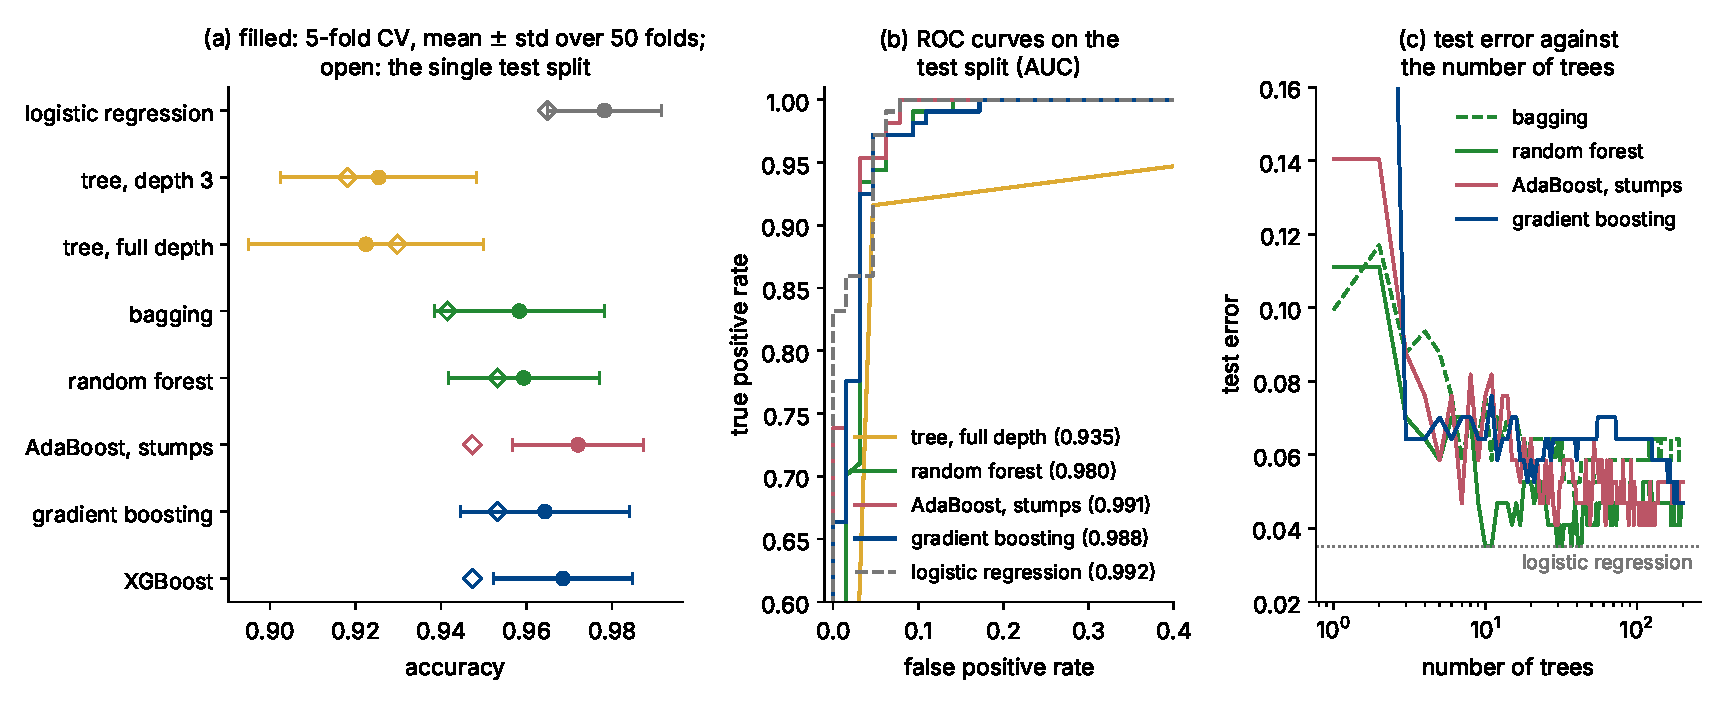
\includegraphics[width=0.94\textwidth]{week48_cancer.pdf}

\footnotesize
\begin{columns}[T]
\begin{column}{0.32\textwidth}
\textbf{(a)} Each step of the ladder moves the cross-validated accuracy up:
trees $0.92$, averaged trees $0.96$, boosted trees $0.96$--$0.97$.  The
error bars are as large as the steps between neighbours.
\end{column}
\begin{column}{0.32\textwidth}
\textbf{(b)} A full tree outputs only 0 or 1 and has a one-point ROC curve;
the ensembles output graded probabilities.  Of the 107 benign tumours in the
test split the tree flags 9 as malignant, the forest 4, logistic regression
2.
\end{column}
\begin{column}{0.32\textwidth}
\textbf{(c)} With some ten to fifty trees every ensemble has done most of
what it can do here.  After that the curves move by one test sample at a
time ($1/171=0.006$).
\end{column}
\end{columns}
\end{frame}

\begin{frame}{Reading the classification ladder}
\begin{columns}[T]
\begin{column}{0.5\textwidth}
\small
\begin{enumerate}
  \item \textbf{One tree $\to$ many trees} is the big step: five and a half
    points of accuracy down to two against the reference.  Deeper single
    trees do not help -- depth 3 and full depth are equal within the noise.
  \item \textbf{Forest against bagging}: a small gain, as the correlation
    between the trees only fell from $0.81$ to $0.78$ (week 46).
  \item \textbf{Boosting} is on top among the trees, with stumps:
    additive effects of single features are enough.
  \item \textbf{Logistic regression wins.}  The classes are close to
    linearly separable in the 30 scaled features; a model with 31 parameters
    and low variance is the right tool for 569 samples.
\end{enumerate}
\end{column}
\begin{column}{0.48\textwidth}
\small
\begin{block}{Accuracy is not the whole story}
\footnotesize
\begin{itemize}
  \item \textbf{Logloss}: full tree $2.53$, forest $0.33$, XGBoost $0.14$,
    logistic regression $0.09$.  A tree that is wrong is wrong with
    probability one.
  \item \textbf{AdaBoost}: AUC $0.991$ but logloss $0.44$ -- it ranks the
    samples well, its scores are not calibrated probabilities.
  \item For a diagnosis a missed malignant tumour costs more than a false
    alarm.  At threshold $0.5$ every method here misses 3 or 4 of the 64
    malignant ones: read the confusion matrix and choose the threshold, as
    in week 43.
\end{itemize}
\end{block}
\begin{block}{The lesson for Project 3}
\footnotesize
Always include the simplest reasonable model.  ``The boosted model reaches
97\,\%'' means something only next to ``and logistic regression reaches
98\,\%''.
\end{block}
\end{column}
\end{columns}
\end{frame}

\begin{insight}[one split or fifty folds?]
\question{On the test split the random forest has accuracy $0.953$ and
AdaBoost $0.947$.  In the repeated cross-validation AdaBoost has $0.972$ and
the forest $0.959$.  Which method is better on these data, and how sure are
we?  What would you write in a report?}
\answer{On the split the difference is \textbf{one sample} out of 171
($1/171=0.006$), and the binomial standard error of an accuracy of $0.95$ on
171 samples is $\sqrt{0.95\cdot0.05/171}=0.017$: the split cannot rank them.
The cross-validation uses every sample for testing ten times and
\emph{pairs} the methods on the same folds: AdaBoost is ahead by $0.013$ on
average.  The fold-to-fold standard deviation ($0.015$--$0.018$) describes
how much a single fold varies, not the uncertainty of the mean; and the
50 folds overlap, so $\mathrm{std}/\sqrt{50}$ is too optimistic an error
bar.  A fair statement: ``AdaBoost with stumps is $1.3$ points better than
the random forest in repeated 5-fold cross-validation ($0.972\pm0.015$
against $0.959\pm0.018$, standard deviation over folds); a single test split
of 171 samples does not resolve the difference.''}
\end{insight}

%% =====================================================================
\subsection{Regression: the California housing data}
%% =====================================================================

\begin{frame}[fragile]{Regression: the California housing data}
\begin{columns}[T]
\begin{column}{0.44\textwidth}
\footnotesize
\textbf{The data} (Pace and Barry 1997; 1990 US census): 20\,640 districts
(census block groups) in California.  The target is the \textbf{median house
value} of the district in units of 100\,000 dollars (mean $2.07$, standard
deviation $1.15$; capped at $5$, which $4.8\,\%$ of the districts reach).

\medskip
\textbf{Eight features}, all numerical: median income \texttt{MedInc},
median house age \texttt{HouseAge}, rooms and bedrooms per household
\texttt{AveRooms}, \texttt{AveBedrms}, \texttt{Population}, persons per
household \texttt{AveOccup}, \texttt{Latitude}, \texttt{Longitude}.

\medskip
A classical test case for boosting: Hastie, Tibshirani and Friedman use it
in their Chapter 10.
\end{column}
\begin{column}{0.54\textwidth}
\begin{lstlisting}
from sklearn.datasets import fetch_california_housing
from sklearn.model_selection import train_test_split

data = fetch_california_housing()    # downloads once
X, y = data.data, data.target        # (20640, 8)
Xtr, Xte, ytr, yte = train_test_split(
    X, y, test_size=0.25, random_state=2026)
print(Xtr.shape, Xte.shape)          # 15480 and 5160
\end{lstlisting}
\footnotesize
\begin{block}{The protocol}
Everything that is tuned is tuned on the \textbf{training} data: the depth
of the single tree by 5-fold cross-validation, the number of boosting
rounds by early stopping on a validation part of the training data.  The
5\,160 test districts are used once.  We report the root mean squared error
(RMSE, in 100\,000 dollars) and $R^2$.
\end{block}
\end{column}
\end{columns}
\end{frame}

\begin{frame}{The data on the map, and the boxes of a tree}
\centering
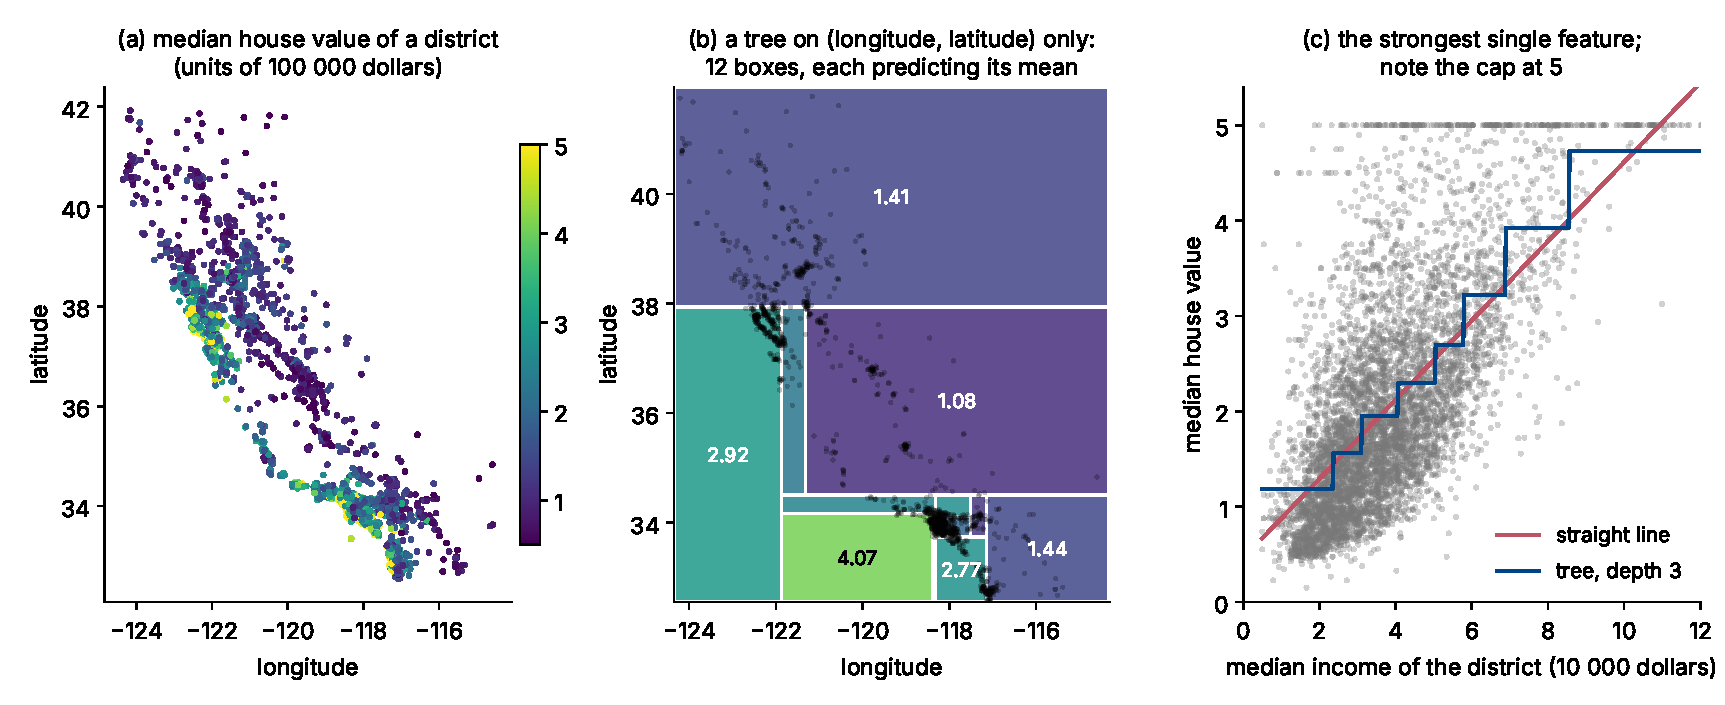
\includegraphics[width=0.96\textwidth]{week48_housing_data.pdf}

\footnotesize
\begin{columns}[T]
\begin{column}{0.32\textwidth}
\textbf{(a)} The expensive districts sit along the coast, around San
Francisco and Los Angeles.  No function of longitude \emph{or} latitude
alone describes that.
\end{column}
\begin{column}{0.32\textwidth}
\textbf{(b)} Recursive binary splitting on the map: the first cut is
latitude $\le37.93$; twelve boxes already find the two metropolitan areas,
test $R^2=0.43$ from the position alone.
\end{column}
\begin{column}{0.32\textwidth}
\textbf{(c)} Income alone gives $R^2=0.48$ with a straight line and with a
depth-3 tree.  The tree is a staircase and flattens at the cap; the line
overshoots it.
\end{column}
\end{columns}
\end{frame}

\begin{frame}{The ladder on the housing data}
\begin{columns}[T]
\begin{column}{0.56\textwidth}
\scriptsize
\setlength{\tabcolsep}{4pt}
\begin{tabular}{@{}lccc@{}}
\toprule
 & \multicolumn{2}{c}{RMSE} & \\
 & train & test & test $R^2$\\
\midrule
linear regression (OLS) & 0.728 & 0.713 & 0.618\\
\midrule
tree, depth 10 (5-fold CV) & 0.480 & 0.647 & 0.686\\
tree, full depth (37) & 0.000 & 0.718 & 0.613\\
\midrule
bagging, 200 deep trees & 0.187 & 0.507 & 0.807\\
random forest, 200 trees, $m=3$ & 0.181 & 0.491 & 0.819\\
\midrule
boosting, depth 3, 200 trees & 0.465 & 0.504 & 0.809\\
boosting, depth 6, 200 trees & 0.293 & 0.467 & 0.836\\
XGBoost, depth 6, early stopping & 0.281 & 0.453 & 0.846\\
\bottomrule
\end{tabular}

\medskip
\footnotesize
The tree of depth 10 has 707 leaves, the full tree 14\,871 -- nearly one
per training district.  Out-of-bag $R^2$: bagging $0.807$, forest $0.819$,
equal to the test $R^2$ to three digits.  Gradient boosting: $\nu=0.1$.
XGBoost: $\nu=0.05$, stopped at $M=703$ trees (patience 50 on $20\,\%$ of
the training data; row and column subsampling $0.8$).
\end{column}
\begin{column}{0.42\textwidth}
\footnotesize
\begin{block}{Reading the table}
\begin{itemize}
  \item A \textbf{fully grown tree} reproduces every training district and
    is no better than a straight line on new ones.
  \item The \textbf{best single tree} (707 leaves) gains a little.
  \item \textbf{Averaging 200 deep trees} takes the same deep trees from
    $0.718$ to $0.507$.
  \item \textbf{Boosting} with depth 6 goes further, $0.453$: a typical
    error of 45\,000 dollars, against 71\,000 for the linear model.
  \item In mean squared error, from $0.508$ (OLS) to $0.205$: a factor
    $2.5$.
\end{itemize}
\end{block}
This time the linear model \textbf{loses clearly}: the position enters
through an interaction of two features, and the income saturates.
\end{column}
\end{columns}
\end{frame}

\begin{frame}{The ladder on the housing data in pictures}
\centering
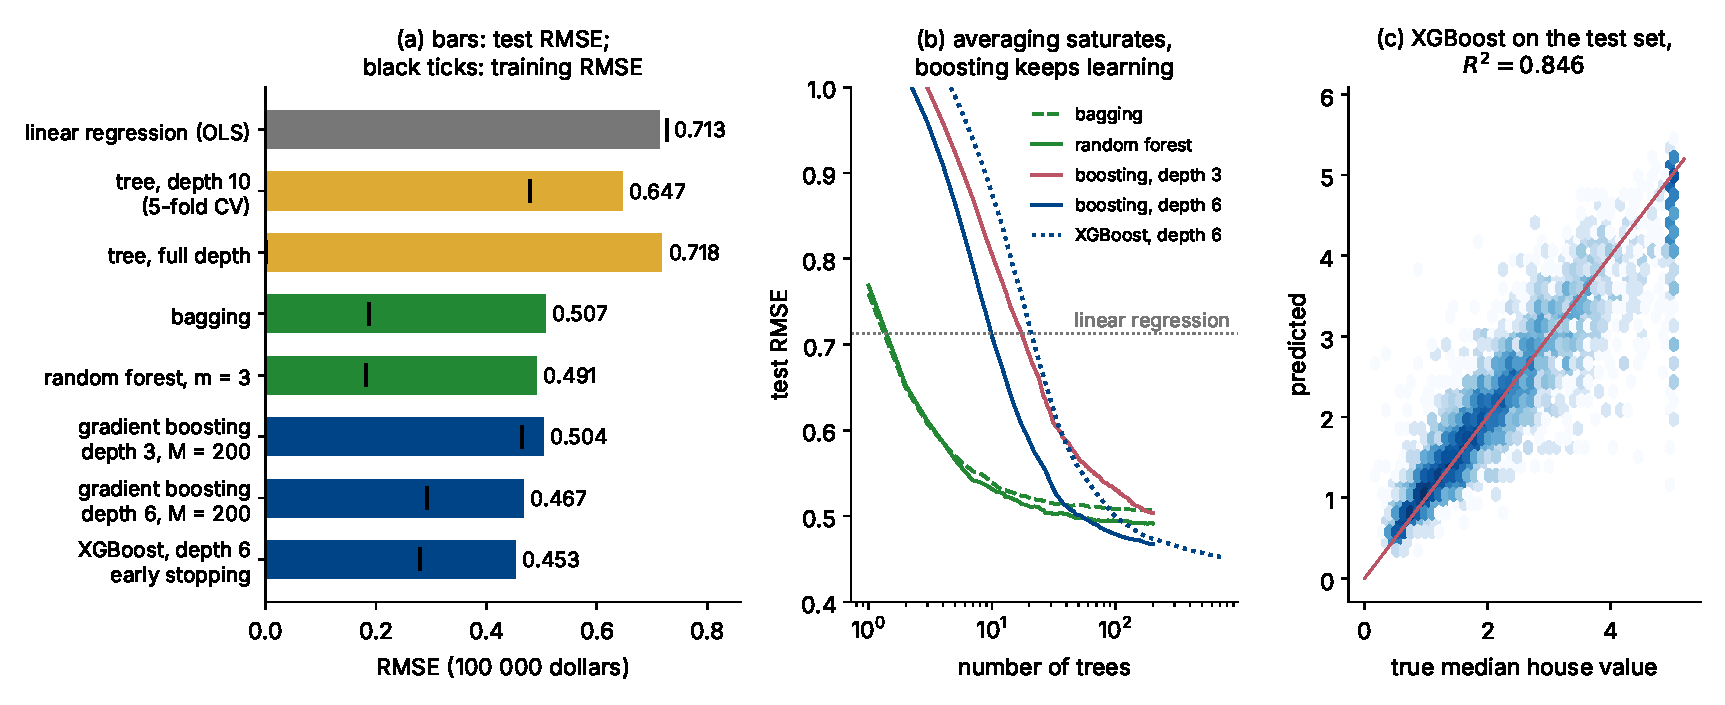
\includegraphics[width=0.96\textwidth]{week48_housing_ladder.pdf}

\footnotesize
\begin{columns}[T]
\begin{column}{0.32\textwidth}
\textbf{(a)} Bars are test errors, black ticks training errors.  Bagging
and the forest fit the training data almost perfectly ($0.18$) and still
generalize; boosting with depth 3 hardly overfits at all.
\end{column}
\begin{column}{0.32\textwidth}
\textbf{(b)} Bagging and the forest are \textbf{flat after about 50
trees} ($0.513\to0.507$, $0.497\to0.491$).  Boosting starts from the mean
(RMSE $1.1$), passes them, and is still falling at 200 trees.
\end{column}
\begin{column}{0.32\textwidth}
\textbf{(c)} Predicted against true value for the 5\,160 test districts.
The vertical stripe at 5 is the cap: districts worth more than 500\,000
dollars were recorded as 500\,001.
\end{column}
\end{columns}
\end{frame}

\begin{frame}{Bias and variance of every step of the ladder, measured}
\centering
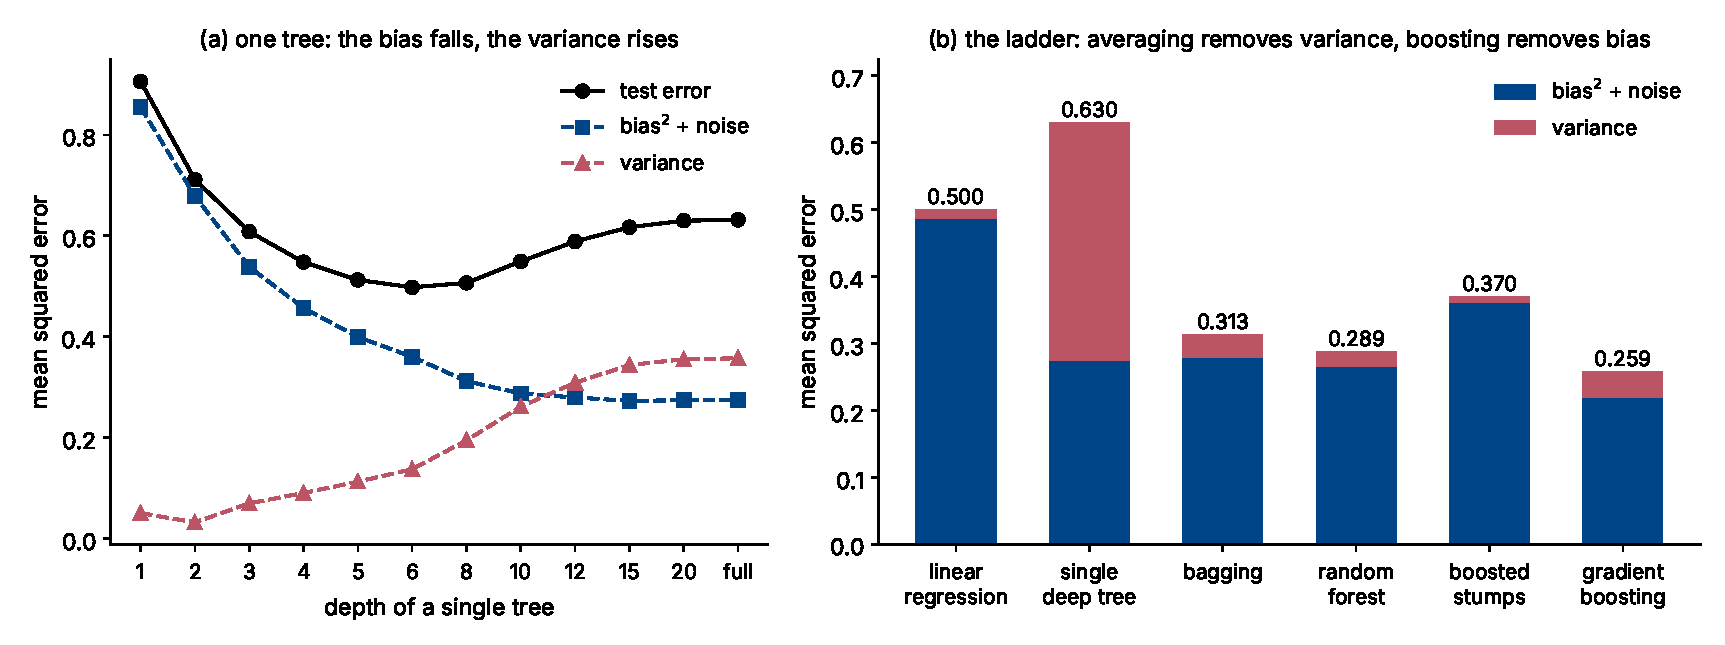
\includegraphics[width=0.9\textwidth]{week48_housing_biasvar.pdf}

\footnotesize
30 training sets of 3\,000 districts, every method fitted on each, all
predicting the same 2\,000 test districts.  With $\bar f$ the prediction
averaged over the training sets, the test error splits exactly as in
Eq.\ (2.52) of week 36,
\[
\underbrace{\overline{(y-f)^2}}_{\text{error}}
=\underbrace{\overline{(y-\bar f)^2}}_{\text{bias}^2+\text{noise}}
+\underbrace{\overline{(f-\bar f)^2}}_{\text{variance}} .
\]
\end{frame}

\begin{frame}{Reading the bias--variance figure: the lecture in six bars}
\begin{columns}[T]
\begin{column}{0.47\textwidth}
\scriptsize
\setlength{\tabcolsep}{4pt}
\begin{tabular}{@{}lccc@{}}
\toprule
 & error & bias$^2$+noise & variance\\
\midrule
linear regression & 0.500 & 0.486 & 0.014\\
tree, depth 1 & 0.906 & 0.855 & 0.051\\
tree, depth 6 & 0.498 & 0.360 & 0.138\\
tree, full depth & 0.630 & 0.275 & 0.355\\
\midrule
bagging, 50 trees & 0.313 & 0.280 & 0.034\\
forest, 50 trees & 0.289 & 0.266 & 0.023\\
\midrule
boosted stumps & 0.370 & 0.361 & 0.009\\
boosting, depth 4 & 0.259 & 0.219 & 0.040\\
\bottomrule
\end{tabular}

\medskip
\footnotesize
Mean squared errors, units $(100\,000\ \text{dollars})^2$; both
boosted models have $M=300$, $\nu=0.1$.  The noise is in
the middle column for every method, so differences in that column are
differences in bias.
\end{column}
\begin{column}{0.51\textwidth}
\footnotesize
\begin{itemize}
  \item \textbf{One tree}: depth trades bias for variance, and the best
    compromise (depth 6, $0.498$) is no better than a straight line.
  \item \textbf{Bagging} keeps the bias of the deep tree ($0.275\to0.280$)
    and divides its variance by ten ($0.355\to0.034$): exactly what
    Eq.\ (7.16) promises, and nothing else.
  \item \textbf{The forest} lowers the variance once more ($0.023$).
  \item \textbf{Boosted stumps} have the variance of a linear model
    ($0.009$) and much less bias ($0.361$ against $0.486$): an additive
    model, one feature at a time.
  \item \textbf{Boosting with depth 4} attacks the bias that averaging
    cannot touch ($0.219$) at a small price in variance.  It wins because
    the bias was the larger term.
\end{itemize}
\end{column}
\end{columns}
\end{frame}

\begin{insight}[what Eq.\ (7.16) says about these trees]
\question{Bagging 50 deep trees reduced the variance from $0.355$ to
$0.034$ -- not to $0.355/50=0.007$.  Use Eq.\ (7.16) to estimate the
correlation $\rho$ between two bagged trees.  What would 5\,000 trees have
given?  And where should the effort go instead?}
\answer{$\rho\sigma^2+(1-\rho)\sigma^2/B=0.034$ with $\sigma^2\approx0.355$
and $B=50$ gives $\rho\approx(0.034-0.007)/0.348\approx0.08$.  With
$B\to\infty$ only the second term disappears: the variance would fall from
$0.034$ to the floor $\rho\sigma^2\approx0.027$, and the error from $0.313$
to about $0.307$.  More trees are almost useless here.  The forest lowers
$\rho$ itself (variance $0.023$ with the same 50 trees).  But the large
term is the \textbf{bias plus noise}, $0.28$: only a different kind of
model -- boosting, $0.22$ -- or better features can reduce that.  (The
estimate is rough: a bootstrap tree sees fewer distinct districts than a
tree on the full sample and has a slightly larger variance.)}
\end{insight}

\begin{frame}{What has the boosted model learned?}
\centering
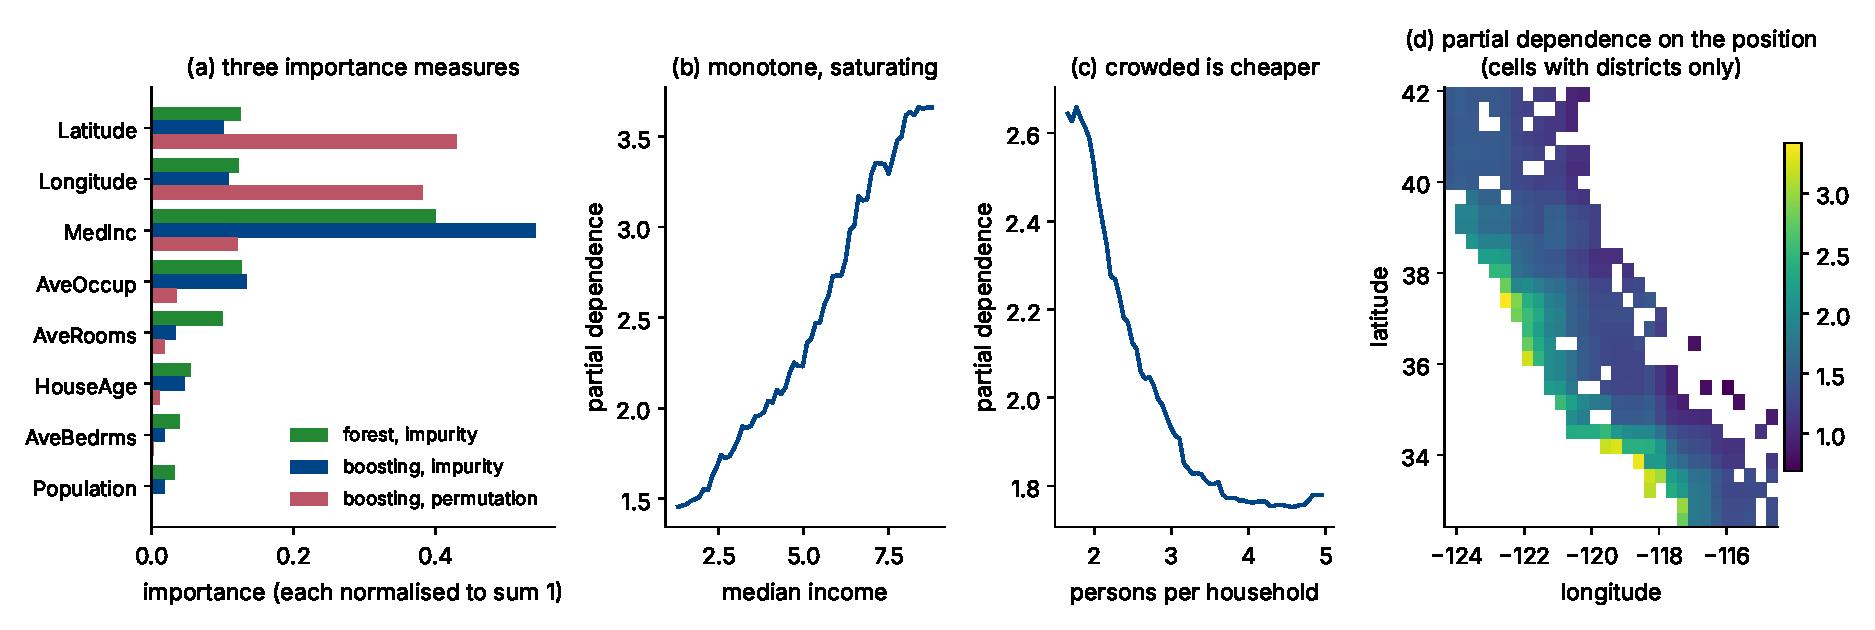
\includegraphics[width=0.93\textwidth]{week48_housing_learned.pdf}

\footnotesize
\begin{columns}[T]
\begin{column}{0.49\textwidth}
\textbf{(a) Importances disagree.}  The impurity importance (the summed
gains of the splits on a feature) puts the income first.  The
\textbf{permutation importance} -- the drop in test $R^2$ when one column
is shuffled -- puts latitude and longitude first ($1.59$ and $1.41$,
against $0.45$ for the income).  The position acts through the \emph{pair}:
shuffling one coordinate moves every district to a wrong place.
\end{column}
\begin{column}{0.49\textwidth}
\textbf{(b)--(d) Partial dependence}: the prediction as a function of one
or two features, averaged over the others.  The value rises from $1.45$ to
$3.66$ with the income and flattens; it falls from $2.6$ to $1.8$ as
households get crowded; (d) redraws the map, with everything else held
fixed.  A model that cannot be read as a tree can still be
\emph{interrogated}.  None of this is causal.
\end{column}
\end{columns}
\end{frame}

\begin{frame}{What to tune, and in which order}
\centering
\scriptsize
\setlength{\tabcolsep}{4pt}
\begin{tabular}{@{}L{2.1cm}L{4.5cm}L{3.0cm}L{3.6cm}@{}}
\toprule
 & the knobs (\texttt{scikit-learn} names) & more trees & start with\\
\midrule
single tree & \texttt{max\_depth}, \texttt{min\_samples\_leaf}, or grow fully and prune
  with \texttt{ccp\_alpha} & -- & cross-validate the depth\\
\addlinespace[1.5pt]
bagging & \texttt{n\_estimators} only & never hurts, saturates & 100--500 deep trees\\
\addlinespace[1.5pt]
random forest & \texttt{max\_features} ($m$); then \texttt{min\_samples\_leaf} &
  never hurts, saturates & $m=\sqrt p$ or $p/3$; check the out-of-bag score\\
\addlinespace[1.5pt]
AdaBoost & \texttt{n\_estimators}, \texttt{learning\_rate}, depth of the weak learner &
  can overfit with noisy labels & stumps, a few hundred rounds\\
\addlinespace[1.5pt]
gradient boosting & \texttt{learning\_rate} ($\nu$) and \texttt{n\_estimators} ($M$)
  \emph{together}; \texttt{max\_depth}; \texttt{subsample} & overfits eventually: stop early &
  $\nu=0.05$--$0.1$, depth 3--6, early stopping\\
\addlinespace[1.5pt]
XGBoost & the same, plus \texttt{reg\_lambda} ($\lambda$), \texttt{gamma} ($\gamma$),
  \texttt{colsample\_bytree}, \texttt{min\_child\_weight} & overfits eventually: stop early &
  the defaults with early stopping, then depth and $\nu$\\
\bottomrule
\end{tabular}

\bigskip
\small
\begin{columns}[T]
\begin{column}{0.48\textwidth}
\textbf{For all of them}: tune with cross-validation or a validation set
taken from the training data (weeks 36 and 44); the out-of-bag score and
early stopping are the two shortcuts the ensembles give us.
\end{column}
\begin{column}{0.48\textwidth}
\textbf{For none of them}: scaling of the features.  A tree only compares a
feature with a threshold.  The linear and neural models in the same
comparison \emph{do} need it -- inside a pipeline.
\end{column}
\end{columns}
\end{frame}

\begin{frame}{Trees and ensembles: what to take with you}
\begin{columns}[T]
\begin{column}{0.5\textwidth}
\small
\begin{enumerate}
  \item A tree is a set of boxes found by a greedy search, Eq.\ (7.9); its
    weakness is variance.
  \item \textbf{Averaging} deep trees removes variance down to
    $\rho\sigma^2$, Eq.\ (7.16); random features lower $\rho$.  Bias is
    untouched.
  \item \textbf{Boosting} adds shallow trees one at a time, each fitted to
    the gradient of a loss: gradient descent in function space.  It removes
    bias, and must be stopped.
  \item On the housing data all of this could be \emph{measured}: variance
    $0.355\to0.034\to0.023$ by averaging, bias plus noise $0.28\to0.22$ by
    boosting.
\end{enumerate}
\end{column}
\begin{column}{0.48\textwidth}
\small
\begin{block}{Two data sets, two outcomes}
\footnotesize
\textbf{Cancer} (569 samples, 30 features): a linear boundary is enough,
logistic regression $0.978$, the best ensemble $0.972$.\\[2pt]
\textbf{Housing} (20\,640 samples, 8 features): interactions and
saturation, boosting reduces the squared error of the linear model by a
factor $2.5$ ($0.508\to0.205$).\\[2pt]
Which method is best is a property of the data, and we find it out by
comparing honestly.
\end{block}
\begin{block}{When to reach for trees}
\footnotesize
Tabular data with mixed, unscaled features and unknown interactions: a
random forest as the baseline that needs no tuning, boosting as the model
to beat.  Images, sequences, differential equations: the networks of weeks
40--45.
\end{block}
\end{column}
\end{columns}
\end{frame}

%% =====================================================================
\section{Lecture 2: summary of the course}
%% =====================================================================

\begin{frame}{}
\centering
{\Large\textbf{Second lecture}}\\[6pt]
{\large Summary of the course: weeks 34 to 47}\\[14pt]
\small What we have covered, what connects it, the insights we want you to
take with you, how to use it -- and what comes after
\end{frame}

\begin{frame}{What? Me worry? No final exam in this course!}
\begin{columns}[c]
\begin{column}{0.4\textwidth}
\centering
\includegraphics[height=0.74\textheight]{exam1.jpeg}
\end{column}
\begin{column}{0.56\textwidth}
\small
\begin{block}{How the course is assessed}
Three projects, each counting one third of the final grade.  Projects 1 and
2 are behind you; \textbf{Project 3 is due Monday December 14} at midnight.
\end{block}
\begin{block}{Project 3, three paths}
\begin{itemize}
  \item[A] neural networks for ordinary and partial differential equations;
  \item[B] a classification problem that is not MNIST, with at least three
    methods -- for example gradient boosting, a dense network and a
    convolutional network;
  \item[C] the statistics and the mathematics of the methods of the
    semester.
\end{itemize}
\end{block}
The rest of this lecture is meant to be useful for all three: it is the map
of what you can draw on.
\end{column}
\end{columns}
\end{frame}

\begin{frame}{Topics we have covered this year}
\begin{columns}[T]
\begin{column}{0.47\textwidth}
\small The course has two central parts.
\begin{block}{Statistical analysis and optimization of data}
\footnotesize
\begin{itemize}
  \item Basic concepts: expectation values, variance, covariance,
    correlation and errors; the central limit theorem.
  \item Central elements of linear algebra: matrix inversion and the
    singular value decomposition, in practice for least squares.
  \item Gradient methods: plain and stochastic gradient descent, momentum,
    AdaGrad, RMSProp and Adam; automatic differentiation.
  \item Estimation of errors and model assessment: the bias--variance
    tradeoff, the bootstrap and cross-validation; confusion matrix, ROC
    curve and AUC for classifiers.
\end{itemize}
\end{block}
\end{column}
\begin{column}{0.51\textwidth}
\begin{block}{Machine learning}
\footnotesize
\begin{itemize}
  \item \textbf{Linear methods for regression and classification}: ordinary
    least squares, Ridge and Lasso regression, logistic regression.
  \item \textbf{Neural networks and deep learning}: feed-forward networks
    and backpropagation, networks for differential equations and
    physics-informed networks, convolutional networks, recurrent networks.
  \item \textbf{Decision trees and ensemble methods}: trees, bagging and
    voting, random forests, boosting and gradient boosting.
\end{itemize}
\end{block}
\begin{block}{Not discussed this year (but in the book)}
\footnotesize
Support vector machines and kernels (Chapter 6); principal component
analysis and autoencoders (Chapter 12); transformers, Boltzmann machines,
variational autoencoders, diffusion models and GANs (Chapters 13--17).
\end{block}
\end{column}
\end{columns}
\end{frame}

\begin{frame}{The semester week by week}
\centering
\scriptsize
\setlength{\tabcolsep}{5pt}
\begin{tabular}{@{}clll@{}}
\toprule
week & Monday lecture & book & projects\\
\midrule
34 & Linear regression: the normal equations, statistics of the estimator & 3.1--3.7 & \\
35 & Ridge and Lasso regression, Gauss--Markov & 3.8--3.11 & \\
36 & The bias--variance tradeoff, bootstrap and cross-validation & Ch.\ 2, 3.14 & \\
37 & Gradient descent and momentum & 4.1--4.6 & \\
38 & Automatic differentiation, AdaGrad, RMSProp, Adam, SGD & Ch.\ 4 & \\
39 & SGD once more, logistic regression, the perceptron & Ch.\ 5 & \\
40 & From logistic regression to the first neural network & Ch.\ 8 & \\
41 & Backpropagation in general, a neural network of our own, MNIST & Ch.\ 8 & \textbf{Project 1}, October 5\\
42 & Neural networks for differential equations, PINNs & Ch.\ 9 & \\
43 & The Poisson equation three ways; reading a classifier; first CNNs & Ch.\ 9, 10 & \\
44 & Convolutional neural networks; cross-validation of a network & Ch.\ 10 & \\
45 & Recurrent neural networks & Ch.\ 11 & \\
46 & Decision trees, bagging and random forests & 7.1--7.10 & \textbf{Project 2}, November 9\\
47 & Boosting: AdaBoost, gradient boosting, XGBoost & 7.11--7.16 & \\
48 & Summary & Ch.\ 18 & \textbf{Project 3}, December 14\\
\bottomrule
\end{tabular}

\smallskip
\footnotesize
Project 1: regression and optimization.  Project 2: neural networks for
regression and classification.  Project 3: your choice among three paths.
\end{frame}

\begin{frame}{Thread 1: every method is the same four choices}
\centering
\scriptsize
\setlength{\tabcolsep}{4pt}
\begin{tabular}{@{}L{2.3cm}L{2.5cm}L{3.0cm}L{2.9cm}L{2.2cm}@{}}
\toprule
 & the model $f(\bm{x};\bm{\theta})$ & the cost function & how it is minimised & the complexity knob\\
\midrule
OLS & $\bm{X}\bm{\theta}$ & mean squared error & closed form: normal equations, SVD & number of features\\
\addlinespace[1.5pt]
Ridge, Lasso & $\bm{X}\bm{\theta}$ & MSE $+\lambda\|\bm{\theta}\|_2^2$ or $+\lambda\|\bm{\theta}\|_1$ &
  closed form (Ridge), gradient methods (Lasso) & $\lambda$\\
\addlinespace[1.5pt]
logistic regression & $\sigma(\bm{x}^T\bm{\theta})$, softmax & cross entropy & gradient descent, SGD, Newton & $\lambda$\\
\addlinespace[1.5pt]
neural networks (dense, CNN, RNN) & layers of affine maps and activations & MSE or cross entropy;
  the residual of an equation (PINNs) & backpropagation $+$ SGD or Adam & width, depth, $\lambda$, epochs\\
\addlinespace[1.5pt]
decision tree & a constant in each of $J$ boxes & Gini, entropy or MSE & greedy recursive splitting & depth, number of leaves\\
\addlinespace[1.5pt]
bagging, random forest & an average of deep trees & that of the trees & bootstrap and average & $m$ (and the trees)\\
\addlinespace[1.5pt]
boosting & a sum of shallow trees & exponential, logistic, squared loss & gradient descent in function space & $M$, $\nu$, depth\\
\bottomrule
\end{tabular}

\medskip
\footnotesize
A method is a \textbf{model}, a \textbf{cost function}, an \textbf{optimizer}
and a way to \textbf{control the complexity} -- ask for these four when you
meet a new one -- and, common to all, a way to \textbf{assess} the result on
data the method has not seen (thread 4).
\end{frame}

\begin{frame}{Thread 2: the bias--variance tradeoff, four times}
\centering
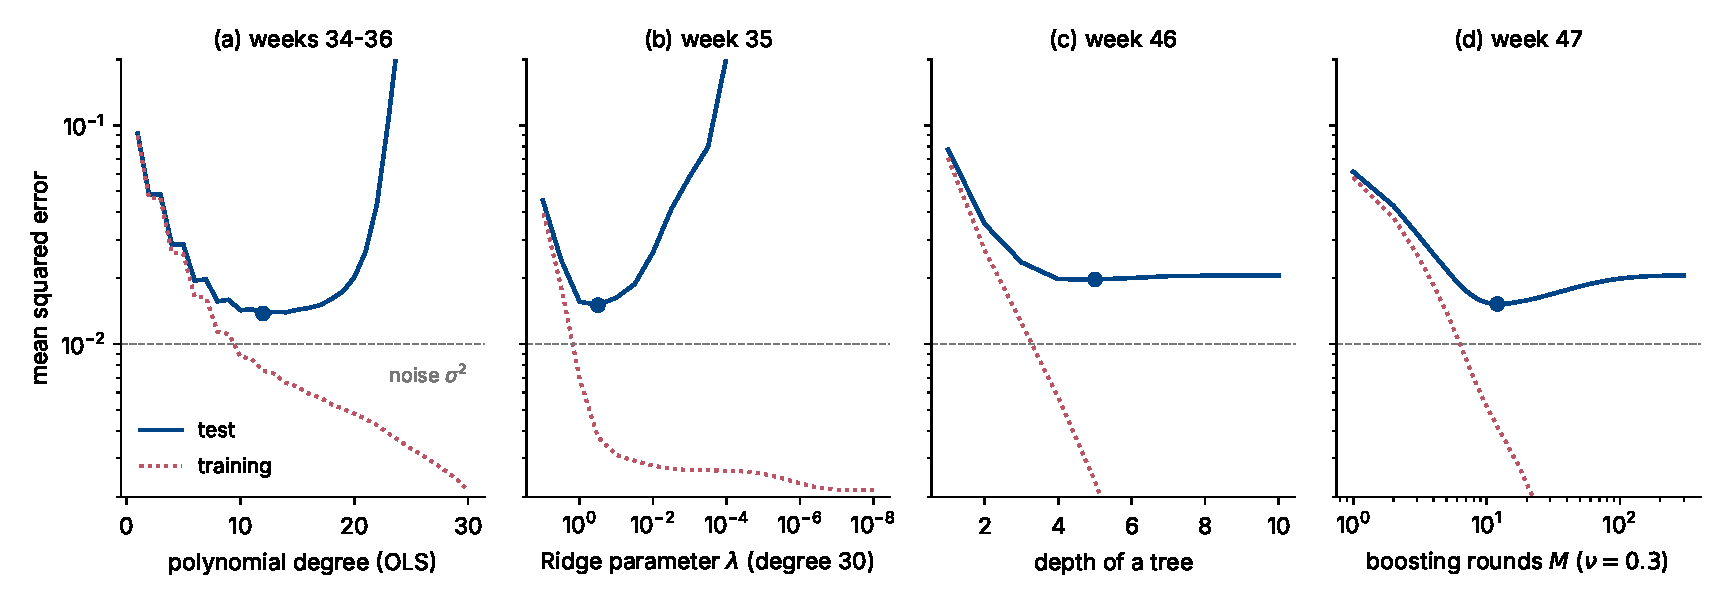
\includegraphics[width=0.88\textwidth]{week48_ucurves.pdf}

\footnotesize
\begin{columns}[T]
\begin{column}{0.55\textwidth}
The noisy Runge function, 40 points, averaged over 100 draws of the noise;
complexity grows to the right.  The training error (dotted) always falls.
The test error, $\mathbb{E}[(y-\tilde y)^2]=\mathrm{bias}^2+\mathrm{variance}+\sigma^2$
(Eq.\ 2.52), has a minimum: degree 12 ($0.0138$), then the polynomial
explodes; $\lambda=0.3$ at degree 30 ($0.0151$); tree depth 5 ($0.0197$);
12 boosting rounds ($0.0152$).  The noise is $\sigma^2=0.01$.
\end{column}
\begin{column}{0.42\textwidth}
\begin{block}{What differs is the price of going too far}
A polynomial of high degree and a vanishing $\lambda$ are catastrophic.  A
fully grown tree and too many boosting rounds are bounded: they reproduce
the noise and cost at most another $\sigma^2$.  That is why averaging deep
trees works -- and why we do not bag polynomials of high degree.
\end{block}
\end{column}
\end{columns}
\end{frame}

\begin{insight}[the same knobs in a neural network]
\question{The four panels have four knobs: the polynomial degree, the Ridge
parameter $\lambda$, the depth of a tree and the number of boosting rounds.
Name the corresponding knobs of a neural network.  Which of them did you
turn in Project 2, and how did you decide where to stop?}
\answer{\textbf{Degree, depth of a tree} $\leftrightarrow$ the number of
hidden nodes and layers: the capacity of the model.  \textbf{Ridge
$\lambda$} $\leftrightarrow$ the same thing, the $L_2$ penalty (weight
decay), and $L_1$ as in Lasso.  \textbf{Boosting rounds} $\leftrightarrow$
the number of epochs: both are steps of a gradient method, and stopping
early is a regularization in both.  The learning rate plays the role of
$\nu$.  In all cases the place to stop is found on data not used for the
fit -- a validation set or cross-validation -- never on the training error,
which only falls, and not on the test set, which is used once.}
\end{insight}

\begin{frame}{Thread 3: gradients, all the way down}
\begin{columns}[T]
\begin{column}{0.5\textwidth}
\small
\begin{enumerate}
  \item \textbf{Set the gradient to zero}: for the mean squared error
    $\nabla C=\frac2n\bm{X}^T(\bm{X}\bm{\theta}-\bm{y})$, and the normal
    equations follow (weeks 34--35).
  \item \textbf{Follow the gradient}:
    $\bm{\theta}\leftarrow\bm{\theta}-\gamma\nabla C$, stable for
    $\gamma<2/\lambda_{\max}$ (Theorem 4.1); momentum, minibatches,
    AdaGrad, RMSProp, Adam (weeks 37--39).
  \item \textbf{Let the computer derive it}: automatic differentiation;
    backpropagation is its reverse mode applied to a network (weeks 38,
    40--41).
\end{enumerate}
\end{column}
\begin{column}{0.48\textwidth}
\small
\begin{enumerate}\setcounter{enumi}{3}
  \item \textbf{Differentiate with respect to the input}: a network
    $u(x,t;\bm{\theta})$ and its derivatives inserted in a differential
    equation, the residual as cost function (weeks 42--43).
  \item \textbf{Differentiate with respect to the function}: the
    pseudo-residuals $-\partial L/\partial f(\bm{x}_i)$ of gradient
    boosting, a tree as the direction, $\nu$ as the learning rate
    (week 47).
\end{enumerate}
\begin{block}{One idea}
\footnotesize
Almost everything we have trained this semester was trained by moving
downhill on a cost function.  The exceptions are instructive: the closed
forms of OLS and Ridge, and the greedy search of a tree -- whose cost
function is not differentiable in its parameters.
\end{block}
\end{column}
\end{columns}
\end{frame}

\begin{frame}{Thread 4: assessing a model honestly}
\begin{columns}[T]
\begin{column}{0.5\textwidth}
\small
\begin{block}{Which data for what}
\footnotesize
\begin{itemize}
  \item \textbf{Training} data to fit; \textbf{validation} data or
    cross-validation to choose hyperparameters; \textbf{test} data once,
    at the end.
  \item Scaling, feature selection and every other data-dependent step
    belong \emph{inside} the fold -- a pipeline.
\end{itemize}
\end{block}
\begin{block}{Resampling: when do we resample?}
\footnotesize
\begin{itemize}
  \item \textbf{Bootstrap}: the uncertainty of an estimate, the
    bias--variance decomposition; reused as a method in bagging, with the
    out-of-bag error as a by-product.
  \item \textbf{$k$-fold cross-validation}: the expected test error, and
    the choice of $\lambda$, depth, learning rate, architecture.
\end{itemize}
\end{block}
\end{column}
\begin{column}{0.48\textwidth}
\small
\begin{block}{Which number}
\footnotesize
\begin{itemize}
  \item Regression: MSE and $R^2$, next to the noise level when it is
    known.
  \item Classification: accuracy next to the majority class; the confusion
    matrix; precision and recall; the ROC curve and the AUC; the cross
    entropy when probabilities matter.
\end{itemize}
\end{block}
\begin{block}{With which uncertainty}
\footnotesize
An accuracy from $n$ test samples has standard error $\sqrt{p(1-p)/n}$; a
cross-validation has a spread over folds; a network has a spread over
seeds.  A difference between two methods smaller than these is not a
result.  Compare on the same folds, and always against a simple baseline.
\end{block}
\end{column}
\end{columns}
\end{frame}

\begin{frame}{One function, the whole semester}
\centering
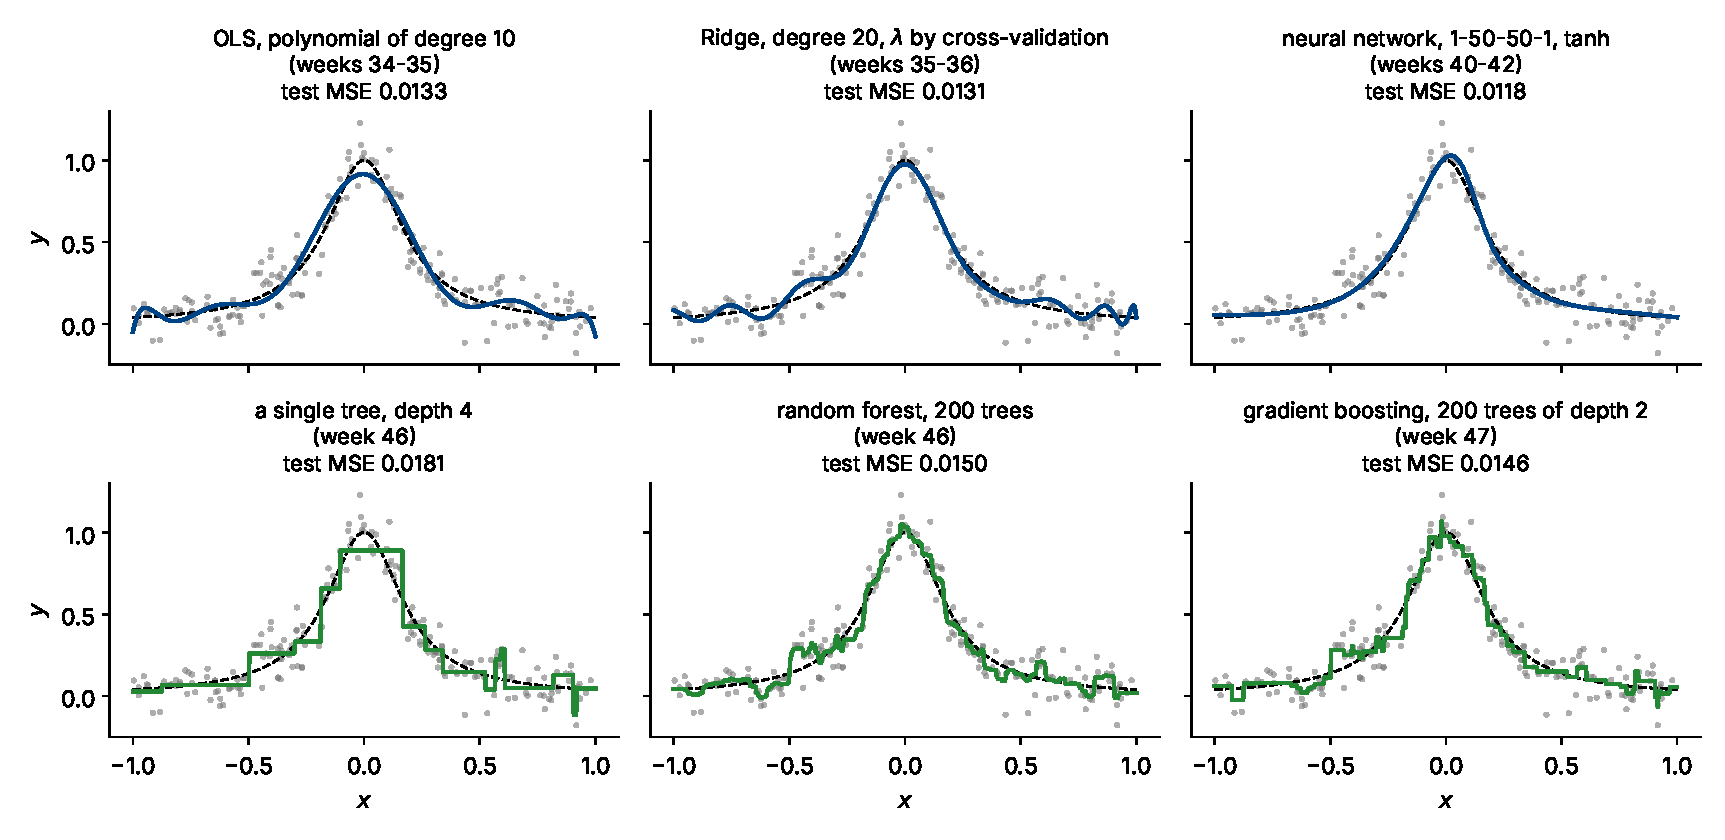
\includegraphics[width=0.84\textwidth]{week48_semester_runge.pdf}

\footnotesize
The noisy Runge function of Project 1 (200 training and 200 test points,
noise variance $0.01$): OLS $0.0133$, Ridge $0.0131$, a neural network
$0.0118$; a tree $0.0181$, a forest $0.0150$, gradient boosting $0.0146$.
A smooth target favours smooth models: sums of trees remain staircases.
\end{frame}

\begin{frame}{One data set, the whole semester: MNIST}
\begin{columns}[T]
\begin{column}{0.52\textwidth}
\scriptsize
\setlength{\tabcolsep}{4pt}
\begin{tabular}{@{}lcl@{}}
\toprule
method (raw pixels) & test acc. & week\\
\midrule
softmax regression & 0.926 & today\\
our own network, 784--100--10 & 0.976 & 41\\
random forest, 100 trees & 0.969 & today\\
gradient boosting, 100 rounds & 0.978 & today\\
convolutional network (PyTorch, Keras) & 0.991 & 44\\
\bottomrule
\end{tabular}

\medskip
\footnotesize
60\,000 training and 10\,000 test images; softmax regression is
multinomial logistic regression, the boosting is \texttt{scikit-learn}'s
histogram version.  The 10\,000 test images give a standard error of about $0.0015$ at these
accuracies: the dense network, the forest and boosting are close to each
other; logistic regression is far below, and the convolutional network far
above.
\end{column}
\begin{column}{0.46\textwidth}
\small
\begin{block}{What the table says}
\footnotesize
\begin{itemize}
  \item Every non-linear method removes some 60 to 70\,\% of the errors of
    the linear one.
  \item Trees on raw pixels do as well as a dense network -- neither knows
    that pixel $(i,j)$ is next to pixel $(i,j+1)$.
  \item The method that \textbf{builds the structure of the data into the
    model} -- locality and shared filters -- removes more than half of the
    remaining errors.
\end{itemize}
\end{block}
\begin{block}{The pattern of the two lectures}
\footnotesize
Cancer data: linear wins.  Housing data: boosted trees win.  Runge
function: smooth models win.  Images: convolutions win.  There is no best
method, only a best method \emph{for a data set}.
\end{block}
\end{column}
\end{columns}
\end{frame}

\begin{frame}{Learning outcomes and overarching aims of this course}
\begin{columns}[T]
\begin{column}{0.54\textwidth}
\small
The course introduces a variety of central algorithms and methods essential
for studies of data analysis and machine learning.  It is project based, and
through the projects you are exposed to fundamental research problems in
these fields, with the aim to reproduce state-of-the-art scientific
results.  You learn to develop and structure larger codes, get acquainted
with computing facilities and learn to handle large scientific projects.  A
good scientific and ethical conduct is emphasized throughout the course.
\end{column}
\begin{column}{0.44\textwidth}
\small
\begin{block}{By now you should}
\footnotesize
\begin{itemize}
  \item understand linear methods for regression and classification;
  \item know neural networks and deep-learning methods;
  \item know trees, bagging and boosting;
  \item master basic data analysis and the assessment of a model;
  \item be able to extend the acquired knowledge to other systems and
    cases;
  \item understand the central algorithms used in data analysis and
    machine learning;
  \item have worked on numerical projects that illustrate the theory -- the
    projects play the central role.
\end{itemize}
\end{block}
\end{column}
\end{columns}
\end{frame}

\begin{frame}{The insights we want you to have after this course}
\begin{columns}[T]
\begin{column}{0.49\textwidth}
\footnotesize
\begin{enumerate}
  \item \textbf{A method is four choices}: a model, a cost function, an
    optimizer and a way to control the complexity.  You can take any new
    method apart in this way.
  \item \textbf{The cost function is derived, not chosen.}  The squared
    error and the cross entropy are maximum likelihood under a model for the
    noise, and the output activation follows from it.
  \item \textbf{Bias and variance are traded, never both removed.}  Every
    method has a knob, the test error has a minimum, and the training
    error does not tell you where it is.
  \item \textbf{The chain rule is enough.}  Gradients drive almost all
    training; automatic differentiation computes them, backpropagation is
    one instance of it -- and a gradient can always be checked.
\end{enumerate}
\end{column}
\begin{column}{0.49\textwidth}
\footnotesize
\begin{enumerate}\setcounter{enumi}{4}
  \item \textbf{Conditioning decides how hard the optimization is.}  The
    learning rate is limited by the largest curvature; scaling the data,
    momentum and adaptive methods all address the same problem.
  \item \textbf{Structure is the cheapest prior.}  Convolutions for images,
    recurrence for sequences, the equation for a physical system, boxes for
    a table: build what you know about the data into the model.
  \item \textbf{A number without an error bar and a baseline is not a
    result.}  Resample, keep the test set for the end, and compare with the
    simplest model that could work.
  \item \textbf{None of it is a black box.}  You have written regression,
    gradient descent and a neural network yourselves and checked them
    against the libraries.  Use that when you read a paper, a code -- or
    the output of a language model.
\end{enumerate}
\end{column}
\end{columns}

\medskip
\small\centering
These eight, more than any single algorithm, are what we hope stays with
you.  The four threads of today are insights 1, 3, 4 and 7.
\end{frame}

%% =====================================================================
\subsection{Practical advice}
%% =====================================================================

\begin{frame}{Starting your machine-learning project}
\begin{columns}[T]
\begin{column}{0.5\textwidth}
\small
\begin{block}{The loop}
\begin{enumerate}
  \item Identify the problem type: classification or regression?
    Supervised at all?
  \item Consider your data carefully.
  \item Choose a \textbf{simple model} that fits 1 and 2, with minimal
    processing of the data.
  \item Consider your data carefully again -- think about how they are
    represented.
  \item Based on your results, go back to the earliest possible point.
\end{enumerate}
\end{block}
\end{column}
\begin{column}{0.48\textwidth}
\small
\begin{block}{Choose a model and an algorithm}
\footnotesize
\begin{itemize}
  \item Start with the simplest model that fits the problem: linear or
    logistic regression.  It is the baseline every later number is read
    against.
  \item Tabular data: then a random forest, then boosting.
  \item Images, sequences, fields: then a network that knows the structure
    -- convolutional, recurrent, physics-informed.
  \item Few data: prefer few parameters, strong regularization, and
    cross-validation over a single split.
\end{itemize}
\end{block}
Today's first lecture was this loop run twice.
\end{column}
\end{columns}
\end{frame}

\begin{frame}{Preparing your data}
\begin{columns}[T]
\begin{column}{0.5\textwidth}
\small
\begin{itemize}
  \item \textbf{Shuffle your data.}  Files are often sorted; minibatches and
    folds must not be.
  \item \textbf{Mean-center your data.  Why?}  The intercept separates from
    the other parameters and is left out of the penalty (week 35); the
    design matrix becomes better conditioned.
  \item \textbf{Normalize the variance.  Why?}  Ridge and Lasso penalize all
    parameters alike, so the features must be comparable; the condition
    number that limits gradient descent falls (week 37); activations do not
    saturate at the start.
\end{itemize}
\end{column}
\begin{column}{0.48\textwidth}
\small
\begin{itemize}
  \item \textbf{Whitening} decorrelates the features as well.  It can be
    hit or miss: it also amplifies directions that are only noise.
  \item \textbf{Trees need none of this}: they are invariant to monotone
    transformations of each feature.
\end{itemize}
\begin{block}{When to do the train/test split?}
\footnotesize
\textbf{First.}  Means, variances, selected features, imputed values: all
are computed from the training data only and then applied to the test data.
Anything else leaks information from the test set into the model, and the
reported error is too small.  In a cross-validation this holds for every
fold -- use a pipeline.
\end{block}
\end{column}
\end{columns}
\end{frame}

\begin{frame}{Neural networks, optimization and hyperparameters}
\begin{columns}[T]
\begin{column}{0.5\textwidth}
\small
\begin{block}{Which activation functions and weights?}
\footnotesize
\begin{itemize}
  \item Hidden layers: ReLU and its relatives (ELU, GELU) for deep
    networks; sigmoid and tanh saturate and their gradients vanish with
    depth -- but tanh is the usual choice in recurrent networks and for
    differential equations, where smooth derivatives are needed.
  \item Output layer: identity for regression, sigmoid for two classes,
    softmax for several -- each with its own cost function, so that the
    output error is simply $\bm{a}^L-\bm{y}$.
  \item All weights zero?  A terrible idea: every node in a layer computes
    the same thing forever.  Small random values, scaled with the number of
    inputs of the layer.
\end{itemize}
\end{block}
\end{column}
\begin{column}{0.48\textwidth}
\small
\begin{block}{Which optimizer?}
\footnotesize
\begin{itemize}
  \item Stochastic gradient descent, with momentum;
  \item adaptive methods: RMSProp, Adam -- a safe first choice, robust to
    the learning rate;
  \item for small problems second-order methods; for boosted trees the
    Newton step is built in.
\end{itemize}
\end{block}
\begin{block}{Which regularization and hyperparameters?}
\footnotesize
$L_1$ or $L_2$, the learning rate, the batch size, the number of epochs,
the architecture; the depth of the trees, the number of rounds.  A large
set to explore: scan the \textbf{learning rate and $\lambda$ on a
logarithmic grid} first, with cross-validation, and report what you
scanned -- as in Project 2.
\end{block}
\end{column}
\end{columns}
\end{frame}

%% =====================================================================
\subsection{Perspectives}
%% =====================================================================

\begin{frame}{Perspective on machine learning}
\begin{columns}[T]
\begin{column}{0.5\textwidth}
\small
\begin{enumerate}
  \item A rapidly emerging application area.
  \item Experiment \emph{and} theory are evolving in many, many fields.
  \item It requires education and retraining for more widespread adoption.
  \item A lot of ``word-of-mouth'' development methods.
  \item And large language models now play a big role here -- also in how
    code and text are written, which is why this course asks you to declare
    how you use them.
\end{enumerate}
\end{column}
\begin{column}{0.48\textwidth}
\small
\begin{block}{An example from physics}
\footnotesize
Huge amounts of data require automation, and classical analysis tools are
often inadequate.  High-energy physics hit this wall in the 1990s.  In 2009
the production of single top quarks was established with \textbf{boosted
decision trees} and Bayesian neural networks, among other methods
(arXiv:0903.0850) -- the methods of the first lecture today.
\end{block}
\begin{block}{Where to find recent results}
\footnotesize
Conference proceedings, arXiv and blog posts: \textbf{NeurIPS}
(\texttt{papers.nips.cc}), \textbf{ICLR} (\texttt{openreview.net}),
\textbf{ICML}; the \emph{Journal of Machine Learning Research}
(\texttt{jmlr.org}); \texttt{arxiv.org/list/cs.LG/recent} and
\texttt{stat.ML}.
\end{block}
\end{column}
\end{columns}
\end{frame}

\begin{frame}{Types of machine learning, a repetition -- and what we left out}
\begin{columns}[T]
\begin{column}{0.5\textwidth}
\small
\begin{block}{By the kind of learning}
\footnotesize
\begin{itemize}
  \item \textbf{Supervised learning}: we know the answer for a set of
    examples and let the computer deduce the logic behind it.  All of this
    course.
  \item \textbf{Unsupervised learning}: finding patterns and relationships
    in data without labels -- clustering, dimensionality reduction,
    generative models.
  \item \textbf{Reinforcement learning}: learning by trial and error, solely
    from rewards and punishments.
\end{itemize}
\end{block}
\begin{block}{By the desired output}
\footnotesize
Classification, regression, clustering -- and generation: a generative
model learns to sample the distribution the data came from.
\end{block}
\end{column}
\begin{column}{0.48\textwidth}
\small
\begin{block}{In the book, not in the lectures}
\footnotesize
\begin{itemize}
  \item Chapter 6: support vector machines and kernel methods.
  \item Chapter 12: principal component analysis and autoencoders.
  \item Chapter 11, second half: LSTM and GRU cells.
  \item Chapter 13: transformers and attention.
  \item Chapters 14--17: generative models -- Boltzmann machines,
    variational autoencoders, diffusion models and normalizing flows,
    generative adversarial networks.
\end{itemize}
\end{block}
\begin{block}{Where these topics are taught}
\footnotesize
The course \textbf{FYS5429}, \emph{Advanced machine learning and data
analysis for the physical sciences}, addresses the topics we have left
out -- all of them \textbf{except support vector machines}, for which
Chapter 6 of the book is the place to go.
\end{block}
\end{column}
\end{columns}
\end{frame}

\begin{frame}{The neural network as a building block}
\small
A neural network is a \textbf{differentiable function with trainable
parameters}, $f(\bm{x};\bm{\theta})$, fitted by backpropagation and a
gradient method to a cost function.  The more advanced methods keep all of
this.  They change \emph{what the network represents} and \emph{where the
training signal comes from}.

\medskip
\centering
\scriptsize
\setlength{\tabcolsep}{4pt}
\begin{tabular}{@{}L{2.5cm}L{3.5cm}L{3.6cm}L{3.6cm}@{}}
\toprule
 & what the network represents & the training signal & what you already know of it\\
\midrule
this course & a regression function, class probabilities, the solution of an equation &
  labelled data: MSE, cross entropy; the residual of the equation &
  everything: weeks 39--45\\
\addlinespace[1.5pt]
transformers & a map from a whole sequence to a sequence: \emph{attention} layers and dense layers, stacked &
  as for any network: a cost function and backpropagation &
  dense layers, softmax, backpropagation, Adam; what recurrent networks struggle with (week 45)\\
\addlinespace[1.5pt]
large language models & the probability of the next token given the text so far -- a transformer &
  the text itself: cross entropy of the next token, no labels needed &
  multiclass classification with softmax, minibatch SGD, weight decay, validation\\
\addlinespace[1.5pt]
reinforcement learning & a \emph{policy} (probabilities of actions) or the \emph{value} of a state and an action &
  rewards collected by acting in an environment &
  softmax output and gradient ascent; regression with the squared error; CNNs that read the state\\
\addlinespace[1.5pt]
generative models (diffusion, VAEs, GANs) & a probability distribution to sample from &
  the data themselves; in diffusion models a regression on added noise &
  MSE regression, maximum likelihood, the bias--variance tradeoff\\
\bottomrule
\end{tabular}
\end{frame}

\begin{frame}{What you already know inside a transformer, a language model and an agent}
\begin{columns}[T]
\begin{column}{0.5\textwidth}
\footnotesize
\begin{block}{Transformers (Chapter 13)}
One block is an attention layer followed by the \textbf{dense network of
week 41}.  Attention is a \textbf{softmax}-weighted average over the
positions of the sequence,
\[
\mathrm{Attention}(\bm{Q},\bm{K},\bm{V})=
\mathrm{softmax}\Big(\frac{\bm{Q}\bm{K}^T}{\sqrt{d}}\Big)\bm{V},
\]
with $\bm{Q},\bm{K},\bm{V}$ affine maps of the input.  All positions are
treated in parallel -- no backpropagation through time.
\end{block}
\begin{block}{Large language models}
A deep transformer trained as a \textbf{classifier}: the classes are the
some $10^5$ tokens of a vocabulary, the cost function is the cross entropy,
$-\sum_t\log p(x_t\,|\,x_1,\dots,x_{t-1};\bm{\theta})$, minimised with
minibatches and a variant of Adam.  New is the scale, not the principle.
\end{block}
\end{column}
\begin{column}{0.48\textwidth}
\footnotesize
\begin{block}{Reinforcement learning}
An agent acts, the environment answers with a new state and a reward.
\begin{itemize}
  \item \textbf{Value-based}: a network $Q(s,a;\bm{\theta})$ fitted by
    least squares to ``reward plus discounted value of the next state'' --
    a \textbf{regression}.  The network that learned Atari games from the
    screen was a CNN trained with RMSProp.
  \item \textbf{Policy-based}: a \textbf{softmax} output gives the
    probabilities of the actions; the parameters follow the gradient of
    the expected reward.
  \item AlphaGo combined both, with CNNs and a tree search.
\end{itemize}
\end{block}
\begin{block}{And together: agentic AI}
A language model that chooses actions -- runs a code, queries a database
-- and receives the result is a policy in a reinforcement-learning loop.
\end{block}
\end{column}
\end{columns}
\end{frame}

\begin{frame}{What is the future like?}
\begin{columns}[T]
\begin{column}{0.5\textwidth}
\small
Deep learning learns directly from raw data and extracts features layer by
layer.  Its success rests on three factors: \textbf{big data, big models,
big computing}.

\begin{block}{Directions, in one line each}
\footnotesize
\begin{itemize}
  \item \textbf{Bayesian machine learning}: a probability distribution
    instead of a number, and with it confidence intervals; priors when data
    are scarce.
  \item \textbf{Reinforcement learning}: agents that act to maximize a
    cumulative reward; AlphaGo (2016) combined it with deep convolutional
    networks.
  \item \textbf{Transfer learning}: knowledge from a source task with much
    data moved to a target task with little.
\end{itemize}
\end{block}
\end{column}
\begin{column}{0.48\textwidth}
\small
\begin{block}{}
\footnotesize
\begin{itemize}
  \item \textbf{Adversarial learning}: two models trained against each
    other, to generate data or to make a model robust.
  \item \textbf{Meta learning}: learning how to learn -- adapting the
    learning method itself to the task.
  \item \textbf{Distributed machine learning}: more than running the same
    algorithm in parallel.
  \item \textbf{Quantum machine learning}: quantum algorithms for linear
    algebra and sampling applied to learning, and machine learning used to
    analyze and control quantum systems.
\end{itemize}
\end{block}
\footnotesize
Chapter 18 of the book has a protocol for a new problem, perspectives
across the sciences (reinforcement learning and foundation models among
them), and a section on what to be sceptical about.
\end{column}
\end{columns}
\end{frame}

\begin{frame}{The challenges facing machine learning}
\begin{columns}[T]
\begin{column}{0.5\textwidth}
\small
\begin{block}{Explainable machine learning}
\footnotesize
We are still at an early stage in explaining why the effective models work
and how.  \textbf{What is missing: the gap between correlation and
causation.}  Most methods -- all of ours -- rely on correlations in the
data.  The partial-dependence curves of the first lecture describe a model,
not a mechanism.
\end{block}
\begin{block}{Cost}
\footnotesize
The computational complexity of the methods is high; lightweight
algorithms and implementations are a research field of their own.
\end{block}
\end{column}
\begin{column}{0.48\textwidth}
\small
\begin{block}{Simple laws instead of complex fits?}
\footnotesize
In physics, chemistry, biology and the social sciences we seek simple
equations -- the Schr\"odinger equation -- that uncover the laws behind the
phenomena.  Can machine learning reveal simple laws instead of ever more
complex models that fit the data?  Physics-informed networks (week 42) are
one step: the equation is put into the cost function.
\end{block}
\begin{block}{Uncertainty}
\footnotesize
A prediction without an error estimate is of limited use in science.  The
bootstrap and cross-validation of this course are the first tools; Bayesian
methods are the systematic answer.
\end{block}
\end{column}
\end{columns}
\end{frame}

\begin{frame}{Other courses on data science and machine learning at UiO}
\begin{columns}[T]
\begin{column}{0.5\textwidth}
\footnotesize
\begin{block}{At the Department of Physics}
\begin{itemize}
  \item \textbf{FYS5429} -- Advanced machine learning and data analysis for
    the physical sciences.  The natural continuation of this course: it
    addresses the topics we have left out, except support vector machines.
  \item \textbf{FYS4425} -- Reinforcement learning and agentic AI for the
    physical sciences.  \textbf{A new course.}
  \item \textbf{FYS5419} -- Quantum computing and quantum machine learning.
\end{itemize}
\end{block}
\begin{block}{Additional courses of interest}
\begin{itemize}
  \item \textbf{STK4051} -- Computational statistics.
  \item \textbf{STK4021} -- Applied Bayesian analysis and numerical methods.
\end{itemize}
\end{block}
\end{column}
\begin{column}{0.48\textwidth}
\footnotesize
\begin{block}{At Mathematics, Informatics and Technology Systems}
\begin{itemize}
  \item \textbf{STK-IN4300} -- Statistical learning methods in data
    science.  An advanced introduction, for students with a good background
    in mathematics and statistics.
  \item \textbf{IN-STK5000} -- Responsible data science.
  \item \textbf{IN4080} -- Natural language processing.
  \item \textbf{IN4310} -- Deep learning for image analysis.
  \item \textbf{IN5310} -- Advanced deep learning for image analysis.
  \item \textbf{IN5490} -- Advanced topics in artificial intelligence for
    intelligent systems.
  \item \textbf{TEK5040} -- Deep learning for autonomous systems.
\end{itemize}
\end{block}
Check the course pages at \texttt{uio.no/studier/emner} for the semester in
which each course is taught.
\end{column}
\end{columns}
\end{frame}

\begin{frame}{The rest of the semester}
\begin{columns}[T]
\begin{column}{0.5\textwidth}
\small
\begin{block}{This week}
\begin{itemize}
  \item \textbf{No Tuesday session.}
  \item \textbf{Wednesday November 25, 12:15--16:00: lab}, dedicated to
    Project 3.  Bring your proposal from week 47, your code and your
    questions.
\end{itemize}
\end{block}
\begin{block}{Project 3}
Deadline \textbf{Monday December 14} at midnight.  The report follows the
format of Project 2; the updated rules for LLMs are at the beginning of the
project text.
\end{block}
\end{column}
\begin{column}{0.48\textwidth}
\small
\begin{block}{What today offers the three paths}
\footnotesize
\begin{itemize}
  \item[A] Thread 3: the gradient with respect to the input, and an honest
    comparison with a standard numerical solution.
  \item[B] The ladder of the first lecture, as code: a baseline, a forest,
    boosting, your networks -- compared on the same folds, with error bars
    and a confusion matrix.
  \item[C] The measured bias--variance decomposition, Eq.\ (7.16) at work,
    the U-curves: each is a template for a study of your own.
\end{itemize}
\end{block}
Everything is in \texttt{week48.ipynb}.
\end{column}
\end{columns}
\end{frame}

\begin{frame}{The last words?}
\centering
\large
Early computer scientist Alan Kay said:\\[10pt]
\textbf{``The best way to predict the future is to create it.''}\\[14pt]
\normalsize
\begin{minipage}{0.78\textwidth}
\small
All machine-learning practitioners, whether scholars or engineers,
professors or students, need to work together to advance these research
topics.  Together we will not just predict the future, but create it.
\end{minipage}
\end{frame}

\begin{frame}{Best wishes to you all, and thanks so much for your heroic efforts this semester}
\centering
\includegraphics[height=0.66\textheight]{Nebbdyr2.png}
\end{frame}

\end{document}
